\documentclass[12pt]{article}
\usepackage{pdfpages}
\usepackage[a4paper, left=15mm, right=15mm, top=20mm, bottom=20mm]{geometry}

% Поддержка русского языка
\usepackage[utf8]{inputenc}
\usepackage[russian]{babel}

\usepackage{amsfonts, amssymb}  
\usepackage{mathtools}
\usepackage{listings} % Для кода
\usepackage{float}    % Для точного позиционирования
\usepackage{hyperref}

\usepackage{cite} % Bibtex


\begin{document}

\thispagestyle{empty}

\begin{center}
  МИНИСТЕРСТВО НАУКИ И ВЫСШЕГО ОБРАЗОВАНИЯ РОССИЙСКОЙ ФЕДЕРАЦИИ \\
  ФЕДЕРАЛЬНОЕ ГОСУДАРСТВЕННОЕ АВТОНОМНОЕ ОБРАЗОВАТЕЛЬНОЕ УЧРЕЖДЕНИЕ ВЫСШЕГО ОБРАЗОВАНИЯ \\
  «НОВОСИБИРСКИЙ НАЦИОНАЛЬНЫЙ ИССЛЕДОВАТЕЛЬСКИЙ ГОСУДАРСТВЕННЫЙ УНИВЕРСИТЕТ» \\
  (НОВОСИБИРСКИЙ ГОСУДАРСТВЕННЫЙ УНИВЕРСИТЕТ, НГУ)
\end{center}

\vspace{1.5cm}

\noindent % Отменяем отступ первой строки
Факультет \hfill Механико-математический \par

\vspace{1cm}

\noindent
Кафедра \hfill Программирования \par
\noindent
Направление подготовки \hfill Математика и компьютерные науки

\vspace{2cm}

\begin{center}
  \vspace{1em} % Отступ после линии
  {\Large \textbf{РЕФЕРАТ}} % Заголовок крупным и жирным шрифтом
  \vspace{1em} % Отступ перед линией
\end{center}

% \vspace{0.5cm}

\begin{center}
  \textbf{Пьянзин Богдан Олегович}
  \rule[0.5ex]{\linewidth}{0.4pt}
  \small (Фамилия, Имя, Отчество автора)
\end{center}

\vspace{1.5cm}

\noindent Тема: Методы адаптивного планирования запросов в реляционных СУБД

% \vfill % Растягиваем вертикальное пространство, чтобы следующий блок был ниже
\vspace{1.5cm}

% --- Блок утверждения и научного руководителя ---
\hspace*{\fill} % Убедимся, что minipage начнется от правого края
\begin{minipage}[t]{0.5\textwidth}
  \textbf{«Реферат принят»}
  
  \vspace{0.5cm} % Отступ
  
  \textbf{Научный руководитель}
  
  \vspace{0.5cm} % Отступ
  
  % Детали руководителя (можно выровнять по левому краю относительно центра или просто слева)
  % Здесь просто слева, но с небольшим отступом от центральной линии
  к.ф-м.н., с.н.с., \\
  старший преподаватель \\
  кафедры программирования ММФ
  
  \vspace{1cm} % Отступ
    % Подпись руководителя (по центру)
  \textbf{Пономарёв Д.К.} / \rule{4cm}{0.4pt} \\ % Фамилия И.О., слэш, линия для подписи
  \small (ФИО, Подпись) % Подсказка мелким шрифтом

  \vspace{1cm} % Отступ

  % Дата
  «\ldots»\makebox[7em]{\dotfill} 2025 г. % День, точки, год, г.
  % «\ldots» мая 2025 г. % День, точки, год, г.
\end{minipage}

\vfill % Растягиваем вертикальное пространство, чтобы последний блок был внизу

% --- Город и Год (по центру внизу) ---
\begin{center}
Новосибирск, 2025
\end{center}


\begin{flushleft}

\newpage


\centering \section*{Оглавление}
\raggedright
\addcontentsline{toc}{section}{Оглавление}

\section*{Введение}
\begin{itemize}
    \item Актуальность темы.
    \item Цель исследования.
\end{itemize}

\section*{Основная часть}

\subsection*{Теоретические основы соединений таблиц в запросах}
\begin{itemize}
    \item Определение и классификация соединений и планирование запроса.
    \item Задача выбора порядка соединений таблиц.
    \item Факторы, влияющие на производительность (размеры таблиц, статистики, индексы, типы данных и т.д.).
\end{itemize}

\subsection*{Методы ускорения перебора соединений таблиц}
\begin{itemize}
    \item Классические подходы.
    \item Реализация в \textbf{PostgreSQL}.
\end{itemize}

\subsection*{Сравнение методов ускорения перебора соединений}
\begin{itemize}
    \item Рекомендации по выбору метода.
\end{itemize}

\section*{Заключение}

\section*{Список источников}
\newpage
%%%%%%%%%%%%%%%%%%%%%%%%%%%%%%%%%%%%%%%%%%%%%%%%%%%%%%%%%%%%
\centering    \section*{Введение}
\centering    \subsection*{Актуальность темы}
\raggedright

Современные СУБД работают с большим объёмом информации и транзакций, используя для ввода запросов язык SQL. 
В процессе трансляции запрос превращается сначала в логическое представление в виде дерева, 
затем с помощью оптимизатора СУБД в физический план исполнения. Производительность СУБД напрямую зависит от качества
построенного физического плана. Для создания "хорошего"\ плана нужно решить или приблизить решение
NP полной задачи перебора соединений таблиц, так как оно требует сложных вычислений и значительных затрат ресурсов.

Сложность задачи обусловлена тем, что количество возможных соединений(бинарных) с n таблицами
равно количеству бинарных деревьев с n листьями - Числа Каталана, которые
имеют экспоненциальную скорость роста.
В классических подходах используется динамическое программирование(DP)
и эвристический поиск для решения этой проблемы. Однако с ростом количества таблиц,
потребление памяти( для хранения промежуточных результатов) и времени планирования становятся
слишком велики. Эвристические методы не гарантируют глобальную оптимальность решения, так как
находят локально оптимальные планы.

Таким образом, выбор неэффективного плана запроса может привести
к значительному замедлению работы системы, а процесс поиска хорошего решения является
нетривиальной задачей. В свою очередь оптимальный план позволяет эффективно исполнить
запрос, с приемлемым потреблением CPU, памяти, I/O, сетевых ресурсов(особенно актуально
для распределённых СУБД).


\centering \subsection*{Цель}
\raggedright
Цель данного исследования – выявить факторы, влияющие на выбор порядка 
соединений в запросах к СУБД, а также рассмотреть классические подходы, применяемые для оптимизации данной задачи.
В рамках работы планируется:
\begin{itemize}
    \item Определить ключевые параметры, влияющие на производительность 
    операций соединения (размер таблиц, наличие индексов, тип соединения и др.).
    \item Разобрать механизмы планирования запросов в \textbf{PostgreSQL}.
    \item Рассмотреть традиционные методы планирования порядка соединений, 
    включая динамическое программирование, эвристические алгоритмы и генетические, 
    используемые в \textbf{PostgreSQL}, изучить их эффективность и ограничения 
    при увеличении числа соединений в запросе.
    \item Выработать критерии для выбора оптимального метода планирования соединений
    в зависимости от типа запроса и структуры данных.
\end{itemize}

Исследование позволит оценить, какие подходы обеспечивают наилучшую 
производительность SQL-запросов в различных условиях и предложить рекомендации 
по их применению. 

%%%%%%%%%%%%%%%%%%%%%%%%%%%%%%%%%%%%%%%%%%%%%%%%%%%%%%%%%%%%%%%%%%%%%%%%%%%%%%

\centering \section*{Основная часть}
\centering \subsection*{Теоретические основы соединений таблиц в SQL запросах}
\centering \subsubsection*{Определение и классификация соединений в планировании запроса}
\raggedright
\textbf{Соединение таблиц} -- это операция, которая позволяет объединять данные
из двух и более таблиц по определённому условию. Использование соединений необходимо,
когда информация распределена между несколькими таблицами. В процессе работы оптимизатора,
решается вопрос какой тип соединения использовать, как и в каком порядке соединить таблицы. 
Существуют три типа соединений:
\begin{description}
    \item[Nested Loop Join] -- для каждой строки из левой таблицы выполняется проход по всем строкам 
    правой таблицы и ищутся соответствующие строки по условию соединения. Пусть левая таблица 
    занимает M страниц и имеет m строк, правая N, n соответственно. Имеется 
    варианты NLJ:
    \begin{description}
        \item[Наивный NLJ] -- перебирается каждая строка левой таблицы, 
        сравнивается с каждой из правой. Сложность $O(M+(m*N))$. Работает медленно 
        если таблицы большие, но прост в реализации, эффективен при малых 
        таблицах.
        \item[Индексированный NLJ] -- правая таблица имеет индекс по соединяемому 
        полю. Сложность $O(M+(m*log(n)))$. Может значительно ускорить поиск, если 
        правая таблица большая. Но будет всё ещё медленным если левая таблица 
        большая.
        \item[Блочный поиск] -- улучшенная версия наивного NLJ, при
        ограничении памяти. Пусть доступно B буферов. Загружаем B-2 
        блоков из левой таблицы, 1 буфер для правой таблицы, 1 под результат. 
        Для каждой страницы из из буферов для левой таблицы, проверяем условие 
        с каждой строкой из буфера правой таблицы, проходимся одним буфером по 
        всей правой таблице. Сложность $O(M + [M/(B-2)] * N)$.
    \end{description}
    \item[Merge Join] --  таблицы сортируются по ключу соединения, происходит 
    построчное  слияние таблиц. Очень хорошо работает если таблицы отсортированы 
    и/или есть индекс по ключу, лучше чем NLJ на больших таблицах. 
    Недостатки: потребность в сортировке, нужно память для хранения 
    сортированных таблиц. Сложность $O(\text{стоимость сортировки двух таблиц} + M + N)$.
    \item[Hash Join] -- строится хэш-таблица для меньшей таблицы, перебирается 
    каждая строка в большей таблице и проверяется соответствие в хэш таблице. 
    Сложность $O(M+N)$. Работает хорошо если одна таблица большая другая маленькая и 
    условие на равенство($=$). Недостатки: требует память для хэш-таблицы, плохо 
    работает если условие на есть диапазон.
\end{description}
Перечисленные выше способы соединения имеют разную эффективность, напрямую зависящую
от статистик. Выбор неоптимального типа соединения может привести к значительному 
ухудшению стоимости исполнения плана. Определение нужного типа происходит в процессе
оптимизации, то есть перевода логического дерева в физическое.

\centering \subsubsection*{Задача выбора порядка соединений}
\raggedright

С увеличением количества данных увеличивается и время, необходимое для 
выполнения запросов. Сокращение времени выполнения запросов становится важным 
фактором для удобства и эффективности СУБД. Оптимизатор преобразует запрос в набор планов. 
Каждый план представлен в виде дерева, вершинами 
в которых являются данные из таблиц или результат соединения таблиц по условию, 
в общем случае называется отношением. Рёбра — условия соединения отношений.
При этом операция соединения отношений не ассоциативна, то есть
$(R1 \times R2) \times R3 \neq R1 \times (R2 \times R3)$ по стоимости.
В статье  \cite{LiuChang2024} приводится
пример разной стоимости для двух деревьев соединений.
\begin{center}
    \begin{tikzpicture}\
        \node (root1) {\textbf{Cost:1000}}
            child { node {Loop Join} 
                child { node {Hash Join} 
                    child { node {Table A} }
                    child { node {Table B} }
                }
                child { node {Table C} }
            }
            child { node {Table D} };
    
        \node (root2) [right=6cm of root1] {\textbf{Cost:3000}}
            child { node {Loop Join} 
                child { node {Hash Join} 
                    child { node {Table A} }
                    child { node {Table C} }
                }
                child { node {Table B} }
            }
            child { node {Table D} };
    \end{tikzpicture}
    \end{center}

Выбор в какой последовательности нужно соединить таблицы является задачей выбора 
порядка соединений. Различные планы исполнения для одного и того же запроса возвращают 
одинаковый результат, но время и ресурсы (CPU, память, I/O обращения, возможно 
сетевые ресурсы), необходимые для выполнения запроса, сильно различаются. Поэтому 
выбор оптимального плана позволяет сократить время отклика, минимизировать 
потребление ресурсов и эффективно обрабатывать большие массивы данных, значительно 
повышая удобство работы пользователя.
\newline

    Задача планировщика/оптимизатора — построить наилучший план выполнения. 
Если это не требует больших вычислений, оптимизатор запросов будет перебирать 
все возможные варианты планов, чтобы в итоге выбрать тот, который имеет наименьшую 
стоимость. Например, если для обрабатываемого отношения создан индекс, прочитать 
отношение можно двумя способами. Во-первых, можно выполнить простое последовательное 
сканирование, а во-вторых, можно использовать индекс, т.е есть выбор сканирования зависит 
от статистик. Затем оценивается стоимость 
каждого варианта и выбирается самый дешёвый, который отдаётся исполнителю(ям).
\centering \subsubsection*{Факторы влияющие на производительность}
\raggedright

Исходя из классификации типов соединений при планировании запроса нужно иметь 
статистику: по размеру отношений, подаваемых на вход оператору, наличию индексов, наличие сортировки данных. 
Применение некоторых типов может потребовать дополнительной памяти.
Помимо этого существуют следующие факторы:
\begin{description}
    \item[Кардинальность отношения] -- количество отдельных строк 
    в таблице базы данных. Если таблица большая, выполнение соединения с ней может 
    быть дорогим, если же таблица маленькая, её можно поместить в память (in-memory), 
    и не придётся обращаться к внешней памяти, что может повлиять на стоимость.
    плана.
    \item[Селективность соединения] -- количество строк, оставшихся после фильтрации. 
    Наиболее селективные соединения следуют применять как можно раньше, так стоимость 
    оператора соединения это стоимость дочерних операторов $+$ собственная обработка.
    \item[Селективность столбцов] -- уникальность значений в столбце. 
    Высокая селективность - много уникальных значений, низкая селективность - мало уникальных значений.
    \item[Корреляция столбцов] -- зависимость значений между столбцами. 
    Если данные сильно коррелируют, оптимизатор может дать неправильную оценку 
    оператору соединения. Тогда ошибка распространиться на операторы стоящие выше,
    что приведёт к ошибке в оценке стоимости исполнения всего плана.
    \item[Распределение данных по столбцам] -- оказывает влияние на оценку селективности
    соединения, размера выходного отношения. Зная распределение, оптимизатор может делать предположения, как
    данных хранятся в отношениях:  использовать последовательное
    сканирование или индекс для поиска( и нужно ли строить индекс).
\end{description}
%%%%%%%%%%%%%%%%%%%%%%%%%%%%%%%%%%%%%%%%%%%%%%%%%%%%%%%%%%%%%%%%%%%%%%
\centering \subsection*{Методы ускорения перебора соединений таблиц}
\raggedright

СУБД применяют классические подходы к оптимизации 
порядка соединений.
\newline
Классические алгоритмы включают в себя:
\begin{itemize}
\item Методы ДП, выполняющие полный поиск среди всех возможных порядков
соединения, но требуют больших затрат памяти и зачастую имеют плохую
асимптотическую сложность.
\item Эвристические методы, требуют меньших затрат ресурсов по сравнению
с ДП, но находят приблизительно (локально) оптимальные планы, а могут также получать и неоптимальные.
\end{itemize}

\centering \subsubsection*{Классические подходы}
\raggedright

Основная идея методов ДП в том, чтобы разбить задачу поиска оптимального
порядка на меньшие(по размеру соединяемых отношений) и решить оптимально их. Затем 
объединить в более крупные и так далее, пока не получим оптимальное решение 
для текущего запроса.
\newline
Эвристический поиск по определённому предположению выбирает
"выгодные"\ планы, отсеивая "плохие"\, на каждом шаге. Зачастую это позволяет
получить приблизительно оптимальный план.
\newline
В данной работе рассмотрим следующие алгоритмы ДП: DPsize, DPsub, DPccp и 
DPhyp. А также эвристические алгоритмы GOO(Greedy Operator Ordering) и 
Geqo. Помимо этого разберём как работает планировщик в \textbf{PostgreSQL}.

\centering \subsubsection*{DPsize \cite[стр. 157]{Thomas}} 
\raggedright

Строит оптимальное \textbf{ветвистое дерево} ( такое дерево, что хотя бы у одной вершины,
начиная с корня, оба потомка составные отношения, т.е не являются таблицами)
снизу вверх, начиная с маленьких соединений и расширяя их. Имеет существенное ограничение -- 
не поддерживает работу с внешними соединениями, т.к их не всегда можно переупорядочивать.


Изначально B хранит каждое отношение $R_i$ как лучший план для $R_i$. 
Затем начинается перебор всех подмножеств размера $\abs{s}$ возможных 
планов от 2 до n. Перебираются всевозможные разбиения S на непересекающиеся 
множества $S_1$, $S_2$, такие что существует хотя бы пара отношений в $S_1$ 
и $S_2$, связанная между собой условием соединения. Так как $\abs{S_1}$ и 
$\abs{S_2}$ меньше $\abs{s}$, то известны их оптимальные планы $p_1$ и $p_2$ соответственно. 
Стоимость объединения $p_1$ и $p_2$ меньше дешевле старой комбинации $S_1$ и 
$S_2$,  то происходит замена.

Сложность DPsize \cite{Moerkotte}:

\begin{align*}
    I^{\text{chain}}_{\text{DPsize}}(n) &=
    \begin{cases}
        \frac{1}{48} (5n^4 + 6n^3 - 14n^2 - 12n), & n \text{ even} \\
        \frac{1}{48} (5n^4 + 6n^3 - 14n^2 - 6n + 11), & n \text{ odd}
    \end{cases}
    \\
    I^{\text{cycle}}_{\text{DPsize}}(n) &=
    \begin{cases}
        \frac{1}{4} (n^4 - n^3 - n^2), & n \text{ even} \\
        \frac{1}{4} (n^4 - n^3 - n^2 + n), & n \text{ odd}
    \end{cases}
    \\
    I^{\text{star}}_{\text{DPsize}}(n) &=
    \begin{cases}
        2^{2n-4} - \frac{1}{4} \binom{2n}{n-1} + q(n), & n \text{ even} \\
        2^{2n-4} - \frac{1}{4} \binom{2(n-1)}{(n-1)} + \frac{1}{4} \binom{(n-1)}{(n-1)/2} + q(n), & n \text{ odd}
    \end{cases}
    \\
    \text{with } q(n) &= n 2^{2n-1} - 5 \times 2^{n-3} + \frac{1}{2} (2^n - 5n + 4)
    \\
    I^{\text{clique}}_{\text{DPsize}}(n) &=
    \begin{cases}
        2^{2n-2} - 5 \times 2^{n-2} + \frac{1}{4} \binom{2n}{n} - \frac{1}{4} \binom{n}{n/2} + 1, & n \text{ even} \\
        2^{2n-2} - 5 \times 2^{n-2} + \frac{1}{4} \binom{2n}{n} + 1, & n \text{ odd}
    \end{cases}
\end{align*}

\begin{algorithm}[H]
    \begin{algorithmic}[1]
        \State \textbf{Input:} A set of relations $R = \{R_1, \dots, R_n\}$ to be joined
        \State \textbf{Output:} An optimal bushy join tree
        \State $B \gets$ an empty DP table $2^R \to$ join tree
        \For{\textbf{each} $R_i \in R$}
            \State $B[\{R_i\}] \gets R_i$
        \EndFor
        \For{\textbf{each} $1 < s \leq n$ \textbf{ascending}}
            \For{\textbf{each} $S_1, S_2 \subset R$ \textbf{such that} $|S_1| + |S_2| = s$}
                \If{(\textbf{not} cross products $\land \neg S_1$ connected to $S_2$) $\lor$ $(S_1 \cap S_2 \neq \emptyset)$}
                    \State \textbf{continue}
                \EndIf
                \State $p_1 \gets B[S_1], p_2 \gets B[S_2]$
                \If{$p_1 = \epsilon$ \textbf{or} $p_2 = \epsilon$} \textbf{continue} \EndIf
                \State $P \gets$ CreateJoinTree($p_1, p_2$)
                \If{$B[S_1 \cup S_2] = \epsilon$ \textbf{or} $C(B[S_1 \cup S_2]) > C(P)$}
                    \State $B[S_1 \cup S_2] \gets P$
                \EndIf
            \EndFor
        \EndFor
    \end{algorithmic}
\end{algorithm}

Где \textbf{chain} - запросы соединения от n таблиц, имеющие вид цепочки. 
\textbf{Cycle, star, clique} -- цикл, звезда(одна вершина связана со многими, все остальные
между собой не имеют связей), полный граф.
%%%%%%%%%%%%%%%%%%%%%%%%%%%%%%%%%%%%%%%%%%%%%%%%%%%%%%%%%%%%%%%%%%%%%%%%%%%%%%%%%%%%%%%%%%%%%%%%
\centering \subsubsection*{DPsub \cite[стр. 158]{Thomas}} 
\raggedright
\begin{algorithm}[H]
    \begin{algorithmic}[1]
        \State \textbf{Input:} A set of relations $R = \{R_1, \dots, R_n\}$ to be joined
        \State \textbf{Output:} An optimal bushy join tree
        \State $B \gets$ an empty DP table $2^R \to$ join tree
        \For{\textbf{each} $R_i \in R$}
            \State $B[\{R_i\}] \gets R_i$
        \EndFor
        \For{\textbf{each} $1 < i \leq 2^n - 1$ \textbf{ascending}}
            \State $S \gets \{ R_j \in R \mid ( \lfloor i / 2^{j-1} \rfloor \mod 2) = 1 \}$
            \For{\textbf{each} $S_1, S_2 \subset S$ \textbf{such that} $S_2 = S \setminus S_1$}
                \If{(\textbf{not} cross products $\land \neg S_1$ connected to $S_2$)}
                    \State \textbf{continue}
                \EndIf
                \State $p_1 \gets B[S_1], p_2 \gets B[S_2]$
                \If{$p_1 = \epsilon$ \textbf{or} $p_2 = \epsilon$} \textbf{continue} \EndIf
                \State $P \gets$ CreateJoinTree($p_1, p_2$)
                \If{$B[S] = \epsilon$ \textbf{or} $C(B[S]) > C(P)$}
                    \State $B[S] \gets P$
                \EndIf
            \EndFor
        \EndFor
    \end{algorithmic}
\end{algorithm}
Перебирает всевозможные подмножества таблиц S. Разделение множество S на  $S_1$ и $S_2$, 
так же как в DPsize. Аналогично, имеются лучшие порядки соединений $p_1$ и $p_2$, 
и если дерево, построенное из $p_1$ и $p_2$ дешевле старого варианта то происходит 
замена. Сложность:
\begin{align*}
    I^{\text{chain}}_{\text{DPsub}}(n) &= 2^{n+2} - n^{2} - 3n - 4 \\
    I^{\text{cycle}}_{\text{DPsub}}(n) &= n2^{n} + 2^{n} - 2n^2 - 2 \\
    I^{\text{star}}_{\text{DPsub}}(n) &= 2 \times 3^{n-1} - 2^{n} \\
    I^{\text{clique}}_{\text{DPsub}}(n) &= 3^n - 2^{n+1} + 1
\end{align*}
\centering \subsubsection*{DPccp \cite[стр. 168]{Thomas} \cite{Moerkotte}}
\raggedright
Пусть дан граф соединений G = (V, E).
Введём понятие csg-cmp-pair (S1, S2) -- в графе запроса выделим $S_1$, 
$S_2$ -- связные непересекающиеся подграфы, такие что $S_1 \in V$ , 
$S_2 \in V/S_1$ ( отсутствие пересечения) и существует между ними ребро. 
$S_1, S_2$ в ($S_1,S_2$) называются комплементарной парой.
\newline

Определим \textbf{csg} -- количество связных подграфов, в определении 
csg-cmp-pair это $S_1$ или $S_2$.
\newline

Определим \textbf{ccp} -- количество csg-cmp-pairs.
\newline

Требуется, чтобы алгоритм обрабатывал все соединения: если 
оператор коммутативен, то для построения плана для $ S_ 1 \cup S_2$ 
из планов для $S_1$ и $S_2$ нужно учитывать коммутативность.

Однако это не представляет особой сложности. Для того, 
чтобы быть корректным, любой алгоритм ДП должен учитывать все csg-cmp-pairs. 
Таким образом, минимальное 
количество вызовов функции стоимости любого алгоритма ДП в точности равно 
количеству csg-cmp-pairs для данного графа. В дальнейшем, в алгоритмах использующих понятие csg-cmp-pair, 
csg будет количеством планов хранимых в DP таблице, как решения 
меньших подзадач. Ccp - будет нижней возможной оценкой алгоритма, 
так как в процессе работы ему нужно обработать все csg-cmp-pairs.
\newline

Заметим, что если $(S_1, S_2)$ - csg-cmp-pair, то и $(S_2, S_1)$
-- тоже. Мы ограничим перечисление csg-cmp-pairs теми $(S_1, S_2)$, 
которые удовлетворяют условию, что $\min(S_1) < \min(S_2)$, 
где $\min(S) = s$ такое, что 
$s \in S$ и $\forall  s^{'} \in  S : s \neq s^{'} \implies  s < s^{'}$. 
Поскольку это ограничение будет действовать для всех csg-cmp-pairs, обработанных алгоритмом, 
не будет вычислено ни одной дублирующей csg-cmp-pair. 
\newline
Теперь задача состоит в том, чтобы перечислить csg-cmp-pairs 
эффективно и в порядке, приемлемом для ДП. 
Задача может быть выражена более конкретно. Перед перечислением csg-cmp-pair $(S_1, S_2)$, 
все csg-cmp-pairs $(S^{'}_1, S^{'}_2)$, где $S^{'}_1 \subseteq  S_1$ 
и $S^{'}_2 \subseteq  S_2$ должны быть пронумерованы.

Сначала алгоритм инициализирует начальные значения $B[{R_i}] = R_i$.
Затем перебираются такие подмножества вершин $S_1$ и $S_2$, 
что $(S_1, S_2)$ -- csg-cmp-pair и $B[S_1]$, $B[S_2]$ уже известны. 
Берутся оптимальные планы $p_1$ и $p_2$ от $S_1$ и $S_2$, затем они 
соединяются. Если стоимость получившегося плана больше B[S], то 
происходит замена. Ограничения:
\begin{itemize}
    \item Не поддерживаются внешние соединения, из-за разбиения на csg-cmp-pairs.
    \item Сильная зависимость алгоритма от эффективности поиска csg-cmp-pair.
\end{itemize}

\begin{algorithm}[H]
    \begin{algorithmic}[1]
        \State \textbf{Input:} A set of relations $R = \{R_1, \dots, R_n\}$
        \State \textbf{Output:} An optimal bushy join tree
        \State $B \gets$ an empty DP table $2^R \to$ join tree
        \For{\textbf{each} $R_i \in R$}
            \State $B[\{R_i\}] \gets R_i$
        \EndFor
        \For{\textbf{each} csg-cmp-pairs $(S_1,S_2)$, S = $S_1 \cup  S_2$}
            \State $p_1 \gets B[S_1], p_2 \gets B[S_2]$
            \State $P \gets$ CreateJoinTree($p_1, p_2$)
            \If{$B[S] = \epsilon$ \textbf{or} $C(B[S]) > C(P)$}
                \State $B[S] \gets P$
            \EndIf
        \EndFor \\
        \textbf{return} $B[\{R_0, \dots, R_{n-1}\}]$
    \end{algorithmic}
\end{algorithm}

Данная реализация возможна, только если удастся перечислить все 
csg-cmp-pairs, т.к DPccp перебирает только связные графы и их комплементарные пары.
Нужно выполнить несколько задач: 
\begin{itemize}
    \item Эффективно пронумеровать все csg.
    \item Не пересчитывать csg дважды, пример (S1, S2) и (S2, S1).
    \item Эффективно находить ccp для каждой csg.
\end{itemize}

Предварительно проведём поиск в ширину и пронумеруем все вершины:

$V = {R_0, \dots,R_{n-1}}$.
Пусть G = {V, E} -- граф запроса.
Введём множества $B_i = \{v_j | j <= i\}$ и функцию соседства 
$N(V^{'}) = \{v^{'} | v \in V^{'} и (v,v^{'}) \in E\}$ , 
чтобы избавиться от повторного добавления $(S_1, S_2)$ и $(S_2, S_1)$
\newline

\begin{algorithm}
    Algorithm EnumerateCsg
    \begin{algorithmic}[1]
        \For{$i = n - 1$ \textbf{to} $0$}  
            \State \textbf{emit} $u_i$; -- Добавим вершины
            \State EnumerateCsgRec($G, u_i, B_i$);
        \EndFor
        \State EnumerateCsgRec($G, S, X$);
        \State $N \gets \mathcal{N}(S) \setminus X$;
        \For{\textbf{each} $S^{'} \subseteq N$ \textbf{where} $S^{'} \neq \emptyset$}
            \State \textbf{emit} $(S \cup S^{'})$ -- Добавим подграф
        \EndFor 
        \For{\textbf{each} $S^{'} \subseteq N$ \textbf{where} $S^{'} \neq \emptyset$}
            \State EnumerateCsgRec($G, (S \cup S^{'}), (X \cup N)$)
        \EndFor 
    \end{algorithmic}
\end{algorithm}

\begin{center}
    \begin{tikzpicture}
        \node (R0) at (0,2) {$R_0$};
        \node (R1) at (-1,1) {$R_1$};
        \node (R2) at (0,1) {$R_2$};
        \node (R3) at (1,1) {$R_3$};
        \node (R4) at (0,0) {$R_4$};

        \draw (R0) -- (R1);
        \draw (R0) -- (R2);
        \draw (R0) -- (R3);
        \draw (R1) -- (R4);
        \draw (R2) -- (R4);
        \draw (R2) -- (R3);
    \end{tikzpicture}
\end{center}

\begin{center}
    \renewcommand{\arraystretch}{1.3} % Увеличиваем высоту строк
    \begin{tabular}{|c|c|c|c|}
        \hline
        \textbf{\textit{S}} & $X$ & $N$ & emit$/S$ \\ 
        \hline
        $\{4\}$ & $\{0,1,2,3,4\}$ & $\emptyset$ & \\ 
        \hline
        $\{3\}$ & $\{0,1,2,3\}$ & $\{4\}$ & $\{3,4\}$ \\ 
        \hline
        $\{2\}$ & $\{0,1,2\}$ & $\{3,4\}$ & $\{2,3\}$ \\ 
        &  &  & $\{2,4\}$ \\ 
        &  &  & $\{2,3,4\}$ \\ 
        \hline
        $\{1\}$ & $\{0,1\}$ & $\{4\}$ & $\{1,4\}$ \\ 
        \hline
        $\rightarrow \{1,4\}$ & $\{0,1,4\}$ & $\{2,3\}$ & $\{1,2,4\}$ \\ 
        &  &  & $\{1,3,4\}$ \\ 
        &  &  & $\{1,2,3,4\}$ \\ 
        \hline
        $\{0\}$ & $\{0\}$ & $\{1,2,3\}$ & $\{0,1\}$ \\ 
        &  &  & $\{0,2\}$ \\ 
        &  &  & $\{0,3\}$ \\ 
        \hline
        $\rightarrow \{0,1\}$ & $\{0,1,2,3\}$ & $\{4\}$ & $\{0,1,4\}$ \\ 
        \hline
        $\rightarrow \{0,2\}$ & $\{0,1,2,3\}$ & $\{4\}$ & $\{0,2,4\}$ \\ 
        \hline
        $\rightarrow \{0,3\}$ & $\{0,1,2,3\}$ & $\{4\}$ & $\{0,3,4\}$ \\ 
        \hline
    \end{tabular}
\end{center}


\begin{algorithm}
    Algorithm EnumerateCmp
    \begin{algorithmic}[1]
        \State \textbf{Input:} A connected query graph $G = (V, E)$, a connected subset $S_1$
        \State \textbf{Precondition:} Nodes in $V$ are numbered according to a BFS
        \State \textbf{Output:} Emits all complements $S_2$ for $S_1$ such that $(S_1, S_2)$ is a csg-cmp-pair
        \State $X \gets B_{\min(S_1)} \cup S_1$
        \State $N \gets \mathcal{N}(S) \setminus X$
        \For{\textbf{each} $u_i \in N$ \textbf{by descending} $i$}
            \State \textbf{emit} $u_i$
            \State EnumerateCsgRec($G, \{u_i\}, X \cup N$)
        \EndFor
    \end{algorithmic}
\end{algorithm}

Вместе эти алгоритмы позволяют эффективно находить ccp для каждой csg.
Сложность:
\[
I^{\text{chain}}_{\text{DPсhain}}(n) =
n^3
\]

\[
I^{\text{cycle}}_{\text{DPccp}}(n) =
n^3
\]

\[
I^{\text{star}}_{\text{DPccp}}(n) =
n2^n
\]

\[
I^{\text{clique}}_{\text{DPccp}}(n) =
3^n
\]
Можно заметить, что также как DPsize и DPsub, DPccp не поддерживает внешние соединения.
Однако он на каждом типе графа имеет меньшую сложность и имеет более сложную
реализацию чем DPsize и DPsub.

\centering \subsubsection*{DPhyp \cite{MoeNeu}}
\raggedright

Является улучшенной версией алгоритма DPccp для работы
с внешними соединениями, которые не всегда коммутативны, а значит 
не всегда допускают переупорядочивания -- есть ограничение на порядок исполнения. Это значит, что если
мы сделаем невалидное переупорядочивание операторов соединения, результат изменится.

\begin{center}
    \begin{tikzpicture}
        % Первое дерево
        \node {$\rightouterjoin_{A.x = C.y} $}
            child { 
                node {$\Join_{B.x = A.y}$}
                    child { node {$A$} }
                    child { node {$B$} }
            }
            child { node {$C$} };
    
        % Знак неравенства между деревьями
        \node at (3, -1.2) {\huge $\neq$};
    
        % Второе дерево
        \node at (6, 0) {$\Join_{B.x = A.y}$}
            child { 
                node {$\rightouterjoin_{A.x = C.y}$}
                    child { node {$A$} }
                    child { node {$C$} }
            }
            child { node {$B$} };
    \end{tikzpicture}
\end{center}

При работе с внешними соединениями возникает понятие гиперграфа.

\textbf{Гиперграф} -- пара (V, E), где V -- непустое множество вершин 
и E -- множество гиперрёбер. 
\textbf{Гиперребро} -- неупорядоченная пара (u, v)
непустых подмножеств V$( u \subset V, v \subset V)$, с условием $u \cap v = \emptyset$
Пусть все вершины V линейно упорядочены по отношению <.
\begin{center}
    \begin{tikzpicture}
        \node (R1) at (-2,2) {$R_1$};
        \node (R2) at (-2,0) {$R_2$};
        \node (R3) at (-2,-2) {$R_3$};
        
        \node (R4) at (2,2) {$R_4$};
        \node (R5) at (2,0) {$R_5$};
        \node (R6) at (2,-2) {$R_6$};
        
        % Центральные соединения
        \node (L) at (-1,0) {};
        \node (R) at (1,0) {};
        % Линии
        \draw (R1) -- (R2);
        \draw (R2) -- (R3);
        \draw (R1) -- (L);
        \draw (R3) -- (L);
        
        \draw (R4) -- (R5);
        \draw (R5) -- (R6);
        \draw (R4) -- (R);
        \draw (R6) -- (R);
        
        \draw (L) -- (R);
    \end{tikzpicture}
\end{center}

Пример: 
$R_1.a + R_2.b + R3.c = R_4.d + R_5.e + R_6.f$ . Этому условию соединения 
соответствует гиперребро  $(\{R_1, R_2, R_3\}, \{R_4, R_5, R_6\})$. $V = {R_1, \dots , R_6}$. 
Простые рёбра:  $({R_1}, {R_2}), ({R_2}, {R_3}), ({R_4}, {R_5})$ и 
$({R_5}, {R_6})$. Отшошение линейного порядка : $R_i < R_j \Leftrightarrow  i < j$.

\textbf{Подграф} -- есть гиперграф H(V, E), $V^{'} \subseteq V$ и $E^{'} = \{(u, v) | (u, v) \in E, u \in V^{'} и v \in V^{'}\}$.
Тогда гиперграф $G^{'} = (V^{'}, E^{'})$, порождённый $V^{'}, E^{'}$ будет подграфом.
\newline

\textbf{Связность гиперграфа} — пусть $H$ — гиперграф. $H$ связный, если $|V| = 1$ или существует разбиение $V$ на $V'$ и $V''$ и существует гиперребро $(u, v) \in E$: $u \subseteq V'$ и $v \subseteq V''$, и порождённые $V'$ и $V''$ подграфы связные. Краткое обозначение: \textbf{csg}.

\textbf{Связное дополнение} — $V' \subseteq V$, $V'' \subseteq (V \setminus V')$ и порождённые $V'$ и $V''$ подграфы связные, то $V''$ — связное дополнение $V'$. Краткое обозначение: \textbf{cmp}.

\textbf{Csg-cmp-pair для гиперграфа} — пусть $H = (V, E)$ — гиперграф, а $S_1, S_2$ — два подмножества $V$ такие, что $S_1 \subseteq V$ и $S_2 \subseteq (V \setminus S_1)$ являются связным подграфом и связным дополнением. Если существует гиперребро $(u, v) \in E$ такое, что $u \subseteq S_1$ и $v \subseteq S_2$, то мы называем $(S_1, S_2)$ \textbf{csg-cmp-pair}.

Основная идея \textbf{Dphyp} такая же, как и у \textbf{DPccp}: постепенно расширять \textbf{csg}-графы, беря новые вершины из функции соседства $N$. $N(S, X)$ при исключающем множестве $X$ состоит из всех вершин, достижимых из $S$, которые не входят в $X$. При этом, выбирая подмножества соседства для включения, мы должны рассматривать гиперузел как атомарный экземпляр: либо все его вершины находятся внутри перечисляемого подмножества, либо ни один из них.

Так как гиперузлы могут пересекаться и упорядоченность вершин важна, определим минимальный элемент множества:
\[
\min(S) = \{s \mid s \in S, \forall s' \in S: s \neq s' \Rightarrow s \prec s'\}.
\]

Для определения функции соседства $N(S, X)$ для гиперграфа определим минимальное множество $E^\downarrow$, такое, что для любого гиперребра $(u, v) \in E$ существует гиперребро $(u', v') \in E^\downarrow$, где $u' \subseteq u$ и $v' \subseteq v$.

Но для начала определим множество:
\[
E^{\downarrow'}(S, X) = \{v \mid (u, v) \in E, u \subseteq S, v \cap S = \emptyset, v \cap X = \emptyset\}.
\]
Определим $E^\downarrow (S, X)$ как минимальное множество гиперузлов, такое, что для всех $v \in E^{\downarrow'}(S, X)$ существует гиперузел $v' \in E^\downarrow (S, X)$, такой что $v' \subseteq v$.

Теперь для гиперграфа определим функцию соседства:
N(S, X) = $\bigcup_{v \in E^\downarrow (S, X)} \min(v)$

Перейдём к самому алгоритму DPhyp, основная идея заключается:
\begin{itemize}
    \item Алгоритм строит все \textbf{ccp} путём перечисления связных подграфов, добавляя большие( по отношению <) 
    вершины к подграфам.
    \item Csg и связанные с ними cmp создаются путём рекурсивного обхода гиперграфа.
    \item Во время обходя графа, некоторые вершины запрещены для посещения, чтобы избежать дублирования csg-cmp-pairs.
    \item Csg увеличиваются за счёт ребёр, ведущим к соседним вершинам. Конечная сторона ребра может приводить сразу к 
    нескольким примитивным вершинам, что нарушает рекурсивный рост компонентов. Поэтому
    гиперрёбра интерпретируются как n к 1 рёбра: n рёбер с одной стороны ведут к одной вершине с другой стороны. 
    Затем с этой вершины на конце ребра происходит рекурсивный рост и используется таблица DP, 
    чтобы проверить, достигнуто ли допустимое построение.
\end{itemize}

Алгоритм начинается с Solve, которая инициализирует DP таблицу с 
планами доступа для одиночных отношений, а затем вызывает EmitCsg 
и EnumerateCsgRec для каждого набора, содержащего ровно одно 
отношение.  EnumerateCsgRec отвечает за перечисление csg.
 Для этого она вычисляет соседство и перебирает каждое ее 
 подмножество. Для каждого такого подмножества $S_1$ вызывается 
 EmitCsg -- нужна  для нахождения  подходящего дополнения. 
 Для этого нужно вызвать EnumerateCmpRec, который рекурсивно перечисляет 
 дополнения $S_2$ для найденного ранее csg $S_1$. 
 Пара $(S_1, S_2)$ является csg-cmp-pair. Для каждой такой пары 
 вызывается EmitCsgCmp. Ее основная задача -- рассмотреть 
 план, построенный из планов для $S_1$  и $S_2$.


\begin{algorithm}
    \begin{algorithmic}[1]
        \State Solve()
        \For{each $u \in V$}
            \State dpTabele[${u}$] = plan for u
        \EndFor
        \For{each $u \in V$ descending according to <}
            \State EmitCsg({u}) - process singleton sets
            \State EnumerateCsgRec({u},$B_u$) - expand singleton sets
        \EndFor \\
        return dpTabele[V]
    \end{algorithmic}
\end{algorithm}

\begin{center}
    \begin{tikzpicture}
        \node[gray] at (-3,1) {$R_1$};
        \node[gray] at (-1,1) {$R4$};
        \node[gray] at (1,1) {$R_1$};
        \node[gray] at (3,1) {$R_4$};

        \node[gray] at (-3,0) {$R_2$};
        \node[gray] at (-1,0) {$R_5$};
        \node[gray] at (1,0) {$R_2$};
        \node[gray] at (3,0) {$R_5$};

        \node[gray] at (-3,-1) {$R_3$};
        \node[gray] at (1,-1) {$R_3$};

        \node[draw, rectangle] at (-1,-1) {\textbf{$R_6$}};
        \node[draw, rectangle] at (3,0) {\textbf{$R_5$}};
        \node at (3,-1) {\textit{$R_6$}};

        % Номера 1 и 2
        \node at (-1,-2) {\large 1};
        \node at (2.5,-2) {\large 2};
    \end{tikzpicture}
\end{center}

\begin{center}
    \begin{tikzpicture}
        % Связный подграф (с рамкой)
        \draw (-0.3,0.3) rectangle (1.3,-0.3);
        \node at (0,0) {$R_1$};
        \node at (1,0) {$R_2$};
        \draw (0.2,0) -- (0.8,0);

        % Подпись
        \node[right] at (1.5,0) {связный подграф};

        % Связанное дополнение (пунктир)
        \draw[dashed] (-0.3,-0.8) rectangle (1.3,-1.4);
        \node at (0,-1) {$R_1$};
        \node at (1,-1) {$R_2$};
        \draw[dashed] (0.2,-1) -- (0.8,-1);

        % Подпись
        \node[right] at (1.5,-1) {связанное дополнение};

        % Запрещённый узел (серый)
        \node[gray] at (7,0) {$R_1$};
        \node[right] at (7.5,0) {запрещённый узел};
        \node at (7,-1) {$R_1$};
        \node[right] at (7.5,-1) {разрешённый узел};
    \end{tikzpicture}
\end{center}

В первом цикле инициализируется таблица ДП с планами для одиночных отношений.  
Во втором цикле для каждой вершины графа запросов в порядке убывания (согласно $\prec$)  
вызываются \texttt{EmitCsg} и \texttt{EnumerateCsgRec}.  

Алгоритм вызывает \texttt{EmitCsg}$(\{v\})$ для отдельных вершин $v \in V$,  
чтобы построить все \textbf{csg-cmp-pairs} $(\{v\}, S_2)$ через вызовы  
\texttt{EnumerateCsgCmp} и \texttt{EmitCsgCmp}, где $v \prec \min(S_2)$.  

Это условие подразумевает, что каждая \textbf{csg-cmp-pair} создаётся только один раз,  
и симметричные пары не генерируются.  

Это соответствует одновершинным графам, например, шаг 1 и 2.

Вызовы \texttt{EnumerateCsgRec} расширяют исходное множество $\{v\}$  
в большие множества $S_1$, для которых затем находятся связные подмножества  
его дополнения $S_2$, такие, что $(S_1, S_2)$ приводит к \textbf{csg-cmp-pair}.  

На шаге 2, где \texttt{EnumerateCsgRec} начинается с $R_5$  
и расширяет его до $\{R_5, R_6\}$ на шаге 4  
(шаг 3 — это построение дополнения).

\begin{center}
    \begin{tikzpicture}
        \node[gray] at (-6,3) {$R_1$};
        \node[gray] at (-6,2) {$R_2$};
        \node[gray] at (-6,1) {$R_3$};
        \node[gray] at (-4,3) {$R_4$};
        \node at (-4,2) {$R_5$};
        \node at (-4,1) {$R_6$};
        \node at (-5,0) {\large 2};
        \node[draw, rectangle] at (-4,2) {\textbf{$R_5$}};

        \node[gray] at (-6+4,3) {$R_1$};
        \node[gray] at (-6+4,2) {$R_2$};
        \node[gray] at (-6+4,1) {$R_3$};
        \node[gray] at (-4+4,3) {$R_4$};
        \node at (-4+4,2) {$R_5$};
        \node at (-4+4,1) {$R_6$};
        \node[draw, rectangle] at (-4+4,2) {\textbf{$R_5$}};
        \node[draw, dashed] at (-4+4,1) {\textit{$R_6$}};
        \draw (-4+4,1) -- (-4+4,2);
        \node at (-5+4,0) {\large 3};

        \node[gray] at (-6+8,3) {$R_1$};
        \node[gray] at (-6+8,2) {$R_2$};
        \node[gray] at (-6+8,1) {$R_3$};
        \node[gray] at (-4+8,3) {$R_4$};
        \node at (-4+8,2) {$R_5$};
        \node at (-4+8,1) {$R_6$};
        \draw (-4+8,1) -- (-4+8,2);
        \node at (-5+8,0) {\large 4};
        \draw (-3.5+8,2.5) rectangle (-4.5+8,0.5);
    \end{tikzpicture}
\end{center}

Чтобы избежать дублирования при перечислении, все вершины, которые 
упорядочены перед v согласно < , запрещены при рекурсивном 
расширении. Формально мы определяем это множество как $B_v = \{w | w < v\} \cup {v}$.

\begin{algorithm}
    EnumerateCsgRec($S_1$, X)
    \begin{algorithmic}[1]
        \For{each $N \subseteq \mathcal{N}(S_1, X): N \neq \emptyset$}
            \If{$dpTable[S_1 \cup N]$}
                \State EmitCsg($S_1 \cup N$)
            \EndIf
        \EndFor
        \For{each $N \subseteq \mathcal{N}(S_1, X): N \neq \emptyset$}
            \State EnumerateCsgRec($S_1 \cup N,X \cup \mathcal{N}(S_1, X)$)
        \EndFor
    \end{algorithmic}
\end{algorithm}

Цель \texttt{EnumerateCsgRec} — расширить заданное множество $S_1$,  
которое порождает связный подграф $G$, до большего множества с тем же свойством.  
Для этого рассматривается каждое непустое подходящее подмножество соседств $S_1$.  

Для каждого из этих подмножеств $N$ проверяется,  
является ли $S_1 \cup N$ связной компонентой.  
Это делается с помощью поиска в таблице \texttt{dpTable}.  
Если проверка прошла успешно, то найден новый связный компонент,  
который далее обрабатывается вызовом \texttt{EmitCsg}$(S_1 \cup N)$.  

Затем, на втором этапе, для всех этих подмножеств $N$ соседства 
вызывается \texttt{EnumerateCsgRec} так,  
что $S_1 \cup N$ может быть рекурсивно расширен.  

Причина, по которой сначала вызывается \texttt{EmitCsg},  
а затем \texttt{EnumerateCsgRec}, заключается в том,  
что для того, чтобы иметь последовательность перечислений,  
допустимую для DP,  
сначала должны быть построены меньшие наборы.  

\begin{center}
    \begin{tikzpicture}
        \node[gray] at (-6,3) {$R_1$};
        \node at (-6,2) {$R_2$};
        \node at (-6,1) {$R_3$};
        \node at (-4,3) {$R_4$};
        \node at (-4,2) {$R_5$};
        \node at (-4,1) {$R_6$};
        \node at (-5,0) {\large 12};
        \node[draw, rectangle] at (-6,2) {\textbf{$R_2$}};

        \node[gray] at (-6+4,3) {$R_1$};
        \node at (-6+4,2) {$R_2$};
        \node at (-6+4,1) {$R_3$};
        \node at (-4+4,3) {$R_4$};
        \node at (-4+4,2) {$R_5$};
        \node at (-4+4,1) {$R_6$};
        \node[draw, rectangle] at (-6+4,2) {\textbf{$R_2$}};
        \node[draw, dashed] at (-6+4,1) {\textit{$R_3$}};
        \draw (-6+4,1) -- (-6+4,2);
        \node at (-5+4,0) {\large 13};

        \node[gray] at (-6+8,3) {$R_1$};
        \node at (-6+8,2) {$R_2$};
        \node at (-6+8,1) {$R_3$};
        \node at (-4+8,3) {$R_4$};
        \node at (-4+8,2) {$R_5$};
        \node at (-4+8,1) {$R_6$};
        \draw (-6+8,1) -- (-6+8,2);
        \node at (-5+8,0) {\large 14};
        \draw (-5.5+8,2.5) rectangle (-6.5+8,0.5);
    \end{tikzpicture}
\end{center}

На шаге 12 был построен \texttt{Solve} на $S_1 = \{R_2\}$.  
Соседство состоит только из $\{R_3\}$, так как $R_1$ находится в $X$  
($R_4, R_5, R_6$ тоже не в $X$, так как не достижимы).  

\texttt{EnumerateCsgRec} сначала вызывает \texttt{EmitCsg},  
который создаст присоединяемое дополнение (шаг 13).  
Затем он проверяет $\{R_2, R_3\}$ на связность.  

Соответствующая запись в \texttt{dpTable} была получена на шаге 13.  
Следовательно, этот тест проходит успешно,  
и $\{R_2, R_3\}$ далее обрабатывается рекурсивным вызовом  
\texttt{EnumerateCsgRec} (шаг 14).  

Теперь расширение останавливается, так как соседство $\{R_2, R_3\}$ пусто,  
поскольку $R_1 \in X$.  

\begin{algorithm}
    EmitCsg($S_1$)
    \begin{algorithmic}[1]
        \State X = $S_1 \cup B_{min(S_1)}$
        \State N = $\mathcal{N}(S_1, X)$
        \For{each $u \in N$ descending according to <}
            \State $S_2$ = {u}
            \If{$\exists (u,v) \in E: u \subseteq S_1 \cap v \subseteq S_2$}
                \State EmitCsgCmp($S_1, S_2$)
            \EndIf
            \State EnumerateCmpRec($S_1,S_2,X$)
        \EndFor
    \end{algorithmic}
\end{algorithm}

\texttt{EmitCsg} принимает в качестве аргумента непустое подходящее подмножество $S_1$ из $V$,  
которое порождает связный подграф.  
Его задача — построить все вершины $S_2$, такие,  
что $(S_1, S_2)$ становится \textbf{csg-cmp-pair}.  

Вершины берутся из соседства $S_1$.  
Все вершины, которые упорядочивались до наименьшего элемента в $S_1$  
(охваченного множеством $B_{\min}(S_1)$), удаляются из соседства,  
чтобы избежать дублирования перечислений.  

Поскольку соседство также содержит $\min(v)$  
для гиперрёбер $(u, v)$ с $|v| > 1$,  
то не гарантируется, что $S_1$ соединён с $v$.  
Чтобы избежать построения ложных \textbf{csg-cmp-pairs},  
\texttt{EmitCsg} проверяет их на связность.  

Тем не менее соседство из одной вершины может быть расширено  
до допустимого дополнения $S_2$ к $S_1$.  
Поэтому перед вызовом \texttt{EnumerateCmpRec},  
который выполняет это расширение, такая проверка не требуется.  

\begin{center}
    \begin{tikzpicture}
        \node at (-6,3) {$R_1$};
        \node at (-6,2) {$R_2$};
        \node at (-6,1) {$R_3$};
        \node at (-4,3) {$R_4$};
        \node at (-4,2) {$R_5$};
        \node at (-4,1) {$R_6$};
        \draw (-6,1) -- (-6,2);
        \draw (-6,2) -- (-6,3);
        \node at (-5,0) {\large 20};
        \draw (-5.5,3.5) rectangle (-6.5,0.5);

        \node at (-6+4,3) {$R_1$};
        \node at (-6+4,2) {$R_2$};
        \node at (-6+4,1) {$R_3$};
        \node at (-4+5,3) {$R_4$};
        \node at (-4+5,2) {$R_5$};
        \node at (-4+5,1) {$R_6$};
        \draw (-6+4,1) -- (-6+4,2);
        \draw (-6+4,2) -- (-6+4,3);
        \node at (-5+4,0) {\large 21};
        \draw (-5.5+4,3.5) rectangle (-6.5+4,0.5);
        \node[draw, dashed] at (-4+5,3) {\textit{$R_4$}};

        % Центральные соединения
        \node (L) at (-1,2) {};
        \node (R) at (0,2) {};
        % Линии
        \draw (-6+4,3) -- (L);
        \draw (-6+4,1) -- (L);
        
        \draw (-4+5,3) -- (R);
        \draw (-4+5,1) -- (R);
        
        \draw (L) -- (R);
    \end{tikzpicture}
\end{center}

Шаг 20.  
Текущий набор $S_1 = \{R_1, R_2, R_3\}$, а $N = \{R_4\}$.  
Поскольку нет гиперребра, соединяющего эти два множества,  
вызов \texttt{EmitCsgCmp} не требуется.  

Однако множество $\{R_4\}$ может быть расширено  
до допустимого дополнения, а именно $\{R_4, R_5, R_6\}$.  
Подходящие вершины для дополнения является задачей вызова  
\texttt{EnumerateCmpRec} на шаге 21.  

\begin{algorithm}
    EnumerateCmpRec($S_1, S_2, X$)
    \begin{algorithmic}[1]
        \ForAll{$N \subseteq \mathcal{N}(S_2, X) \colon N \neq \emptyset$}
            \If{$\texttt{dpTable}[S_2 \cup N] \neq \emptyset \;\land$  
                $\exists (u, v) \in E \colon u \subseteq S_1 \;\land\; v \subseteq S_2 \cup N$}
                \State \texttt{EmitCsgCmp}($S_1, S_2 \cup N$)
            \EndIf
        \EndFor
        \State $X \gets X \cup \mathcal{N}(S_2, X)$
        \ForAll{$N \subseteq \mathcal{N}(S_2, X) \colon N \neq \emptyset$}
            \State EnumerateCmpRec($S_1, S_2 \cup N, X$)
        \EndFor
    \end{algorithmic}
\end{algorithm}

\texttt{EnumerateCsgRec} имеет три параметра.  
Первый параметр $S_1$ используется только для передачи его в \texttt{EmitCsgCmp}.  

Второй параметр — это множество $S_2$,  
которое является связным и должно расширяться до тех пор,  
пока не будет достигнута допустимая \textbf{csg-cmp-pair}.  
Поэтому рассматривается соседство $S_2$.  

Для каждого непустого подходящего подмножества $N$ соседства  
проверяется, является ли $S_2 \cup N$ связным подмножеством  
и соединённым с $S_1$.  

Если да, то мы имеем корректную \textbf{csg-cmp-pair} $(S_1, S_2)$  
и можем приступить к построению плана  
(это делается в \texttt{EmitCsgCmp}).  

Независимо от результата проверки,  
мы рекурсивно пытаемся расширить $S_2$,  
так, чтобы эта проверка оказалась успешной.  

В целом, \texttt{EnumerateCmpRec} очень похоже на \texttt{EnumerateCsgRec}.  

\begin{center}
    \begin{tikzpicture}
        \node at (-6,3) {$R_1$};
        \node at (-6,2) {$R_2$};
        \node at (-6,1) {$R_3$};
        \node at (-4+1,3) {$R_4$};
        \node at (-4+1,2) {$R_5$};
        \node at (-4+1,1) {$R_6$};
        \draw (-6,1) -- (-6,2);
        \draw (-6,2) -- (-6,3);
        \node at (-5,0) {\large 21};
        \draw (-5.5,3.5) rectangle (-6.5,0.5);
        \node[draw, dashed] at (-4+1,3) {\textit{$R_4$}};
        \node (L) at (-5,2) {};
        \node (R) at (-4,2) {};
        \draw (-6,3) -- (-5,2);
        \draw (-6,1) -- (-5,2);
        \draw (-4+1,3) -- (-4,2);
        \draw (-4+1,1) -- (-4,2);
        \draw (-5,2) -- (-4,2);

        \node at (-6+5,3) {$R_1$};
        \node at (-6+5,2) {$R_2$};
        \node at (-6+5,1) {$R_3$};
        \node at (-4+1+5,3) {$R_4$};
        \node at (-4+1+5,2) {$R_5$};
        \node at (-4+1+5,1) {$R_6$};
        \draw (-6+5,1) -- (-6+5,2);
        \draw (-6+5,2) -- (-6+5,3);
        \node at (-5+5,0) {\large 22};
        \draw (-5.5+5,3.5) rectangle (-6.5+5,0.5);
        \node[draw, dashed] at (-4+1+5,3) {\textit{$R_4$}};
        \node (L) at (-5+5,2) {};
        \node (R) at (-4+5,2) {};
        \draw (-6+5,3) -- (-5+5,2);
        \draw (-6+5,1) -- (-5+5,2);
        \draw (-4+1+5,3) -- (-4+5,2);
        \draw (-4+1+5,1) -- (-4+5,2);
        \draw (-5+5,2) -- (-4+5,2);

        \node at (-6+10,3) {$R_1$};
        \node at (-6+10,2) {$R_2$};
        \node at (-6+10,1) {$R_3$};
        \node at (-4+1+10,3) {$R_4$};
        \node at (-4+1+10,2) {$R_5$};
        \node at (-4+1+10,1) {$R_6$};
        \draw (-6+10,1) -- (-6+10,2);
        \draw (-6+10,2) -- (-6+10,3);
        \node at (-5+10,0) {\large 23};
        \draw (-5.5+10,3.5) rectangle (-6.5+10,0.5);
        \node[draw, dashed] at (-4+1+10,3) {\textit{$R_4$}};
        \node (L) at (-5+10,2) {};
        \node (R) at (-4+10,2) {};
        \draw (-6+10,3) -- (-5+10,2);
        \draw (-6+10,1) -- (-5+10,2);
        \draw (-4+1+10,3) -- (-4+10,2);
        \draw (-4+1+10,1) -- (-4+10,2);
        \draw (-5+10,2) -- (-4+10,2);
    \end{tikzpicture}
\end{center}

На шаге 21 
$S_1 = \{R_1, R_2, R_3\}$ и $S_2 = \{R_4\}$.  
$N = \{R_5\}$.  

Множество $\{R_4, R_5\}$ порождает связный подграф.  
Он был вставлен в \texttt{dpTable} на одном из прошлых шагов.  
Однако не существует гиперребра, соединяющего его с $S_1$.  
Следовательно, вызов \texttt{EmitCsgCmp} не производится.  

Далее следует рекурсивный вызов на шаге 22  
с изменением $S_2$ на $\{R_4, R_5\}$.  
Его соседством является $\{R_6\}$.  
Множество $\{R_4, R_5, R_6\}$ приводит к связному подграфу.  

Поиск в \texttt{dpTable} находит соответствие,  
так как запись была сделана на шаге 7.  
Вторая часть проверки также успешна,  
так как одно гиперребро соединяет это множество с $S_1$.  

Следовательно, вызов \texttt{EmitCsgCmp} на шаге 23 происходит  
и строит планы, содержащие все отношения.  

\begin{algorithm}
    EmitCsgCmp($S_1, S_2$)
    \begin{algorithmic}[1]
            \State $\text{plan}_1 = \texttt{dpTable}[S_1]$
            \State $\text{plan}_2 = \texttt{dpTable}[S_2]$
            \State $S = S_1 \cup S_2$
            \State $p = \bigwedge_{(u_1, u_2) \in E, u_i \subseteq S_i} \mathcal{P}(u_1, u_2)$
            \State $\text{newplan} = \text{plan}_1 \Join_p \text{plan}_2$
            \If{$\texttt{dpTable}[S] = \emptyset \;\lor\; \text{cost}(\text{newplan}) < \text{cost}(\texttt{dpTable}[S])$}
                \State $\texttt{dpTable}[S] = \text{newplan}$
            \EndIf
            \State $\text{newplan} = \text{plan}_2 \Join_p \text{plan}_1$ \quad // for commutative ops only
            \If{$\text{cost}(\text{newplan}) < \texttt{dpTable}[S]$}
                \State $\texttt{dpTable}[S] = \text{newplan}$
            \EndIf
    \end{algorithmic}
\end{algorithm}

Задача \texttt{EmitCsgCmp}$(S_1, S_2)$ — соединить оптимальные планы  
для $S_1$ и $S_2$, которые должны образовать \textbf{csg-cmp-pair}.  

Для этого мы должны быть в состоянии вычислить  
правильный предикат соединения и затраты на результирующие соединения.  
Для этого необходимо, чтобы предикаты присоединения,  
селективности и кардинальности были привязаны к гиперграфу.  

Поскольку мы скрываем вычисления стоимости  
в абстрактной функции \texttt{cost},  
нам нужно только явно собрать предикат соединения.  

Для данного гиперграфа $G = (V, E)$  
и гиперребра $(u, v) \in E$,  
определим $\mathcal{P}(u, v)$ —  
условие соединения по этому ребру.  

Сначала из таблицы DP  
извлекаются оптимальные планы для $S_1$ и $S_2$.  
Затем мы запоминаем в $S$ общее множество отношений,  
присутствующих в плане, который необходимо построить.  

Предикат соединения $p$ собирается  
путём взятия конъюнкции предикатов тех гиперграниц,  
которые соединяют $S_1$ и $S_2$.  

Затем планы строятся,  
и если они дешевле существующих,  
они сохраняются в \texttt{dpTable}.

\centering \subsubsection*{Обработка внешних соединений}
\raggedright
%%%%%%%%%%%%%%%%%%%%%%%%%%%%%%%%

Введём два понятия из статьи:
\begin{description}
    \item[Syntactic eligibility set (SES)] --  множество таблиц, которые должны быть соединены до того, 
    как можно применить внешнее соединение.
    \item[Total eligibility set (TES)] --  полный список ограничений на порядок , расширяет SES и учитывает все зависимости между соединениями.
    Формирует гиперрёбра, запрещая недопустимые перестановки. 
    Строится на основе SES и обходе логического дерева соединений, проверяя конфликты с другими операторами. Добавляя TES в гиперграф
    можно создавать допустимые рёбра.
\end{description}
Использование гиперграфа позволяет запрещать недопустимые перестановки 
внешних соединений, задавая при этом допустимый порядок соединений 
т.е ненужные рёбра не будут сгенерированы в графе.
%%%%%%%%%%%%%%%%%%%%%%%%%%%%%%%%%%%%%%%%%%
\newline
Таким образом DPhyp, является относительно( DPsize, DPsub) эффективным алгоритмом.
При этом позволяет обрабатывать внешние соединения.

Все раcсмотренные алгоритмы порождали планы в виде ветвистых деревьев, так как они 
в отличие от односторонних деревьев позволяют использовать преимущества параллелизма.
Планы можно выполнить параллельно, если они не зависят друг от друга, т.е 
соединения A и B можно выполнить параллельно, если на любом пути от корня 
до таблицы нет одновременно A и B. Такого нельзя добиться на односторонних 
деревьях.

\begin{figure}[H]
    \centering
    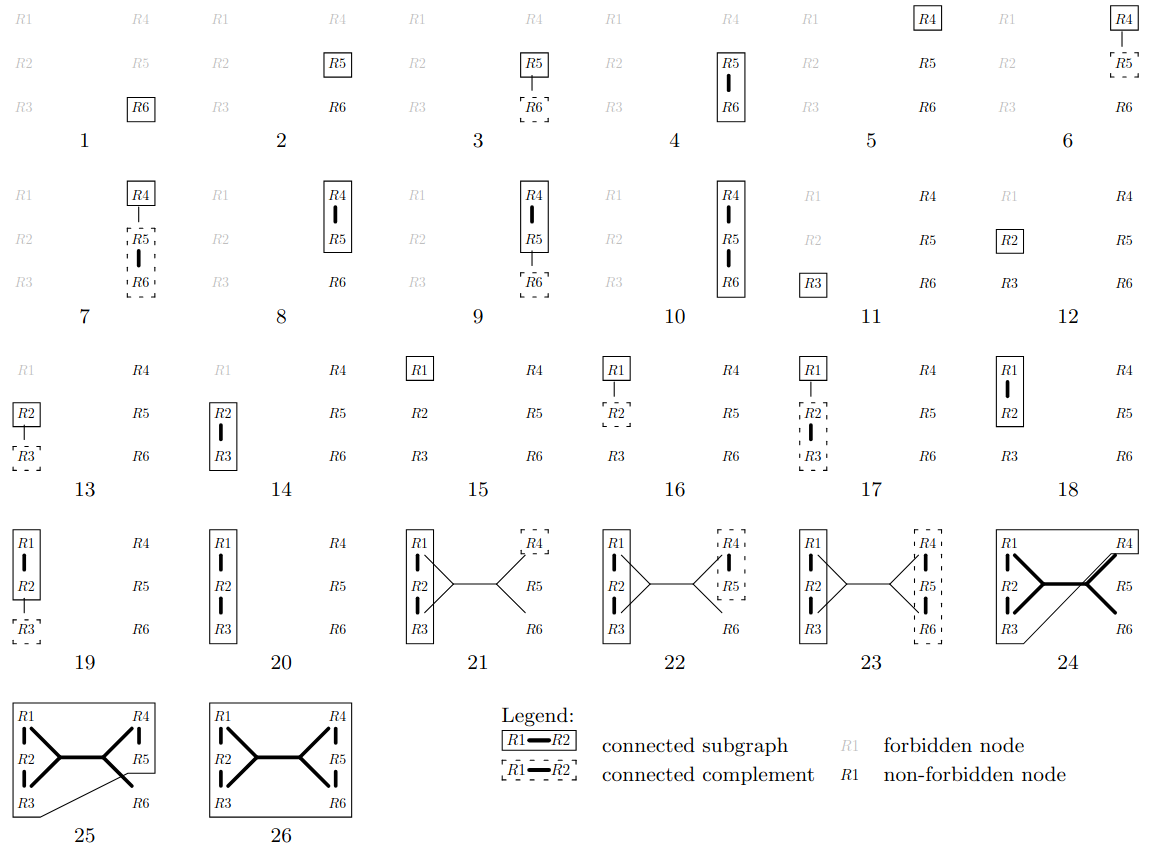
\includegraphics[width=0.8\textwidth]{image.png}
\end{figure}


\centering \subsubsection*{ДП в PostgreSQL}
\raggedright
В PostgreSQL в файле src/backend/optimizer/path/allpaths.c реализованы алгоритмы планирования запросов.
Они применяются в методе:
\begin{lstlisting}
static RelOptInfo *make_rel_from_joinlist(PlannerInfo  *root, List  *joinlist){...}
\end{lstlisting}

Внутри метода есть переменная int $levels\_needed$ -- количество соединяемых таблиц.
Также есть блок кода в котором происходит выбор подхода для оптимизации:
\begin{lstlisting}
    if (join_search_hook)
        return (*join_search_hook) (root, levels_needed, initial_rels);
    else if (enable_geqo && levels_needed >= geqo_threshold)
        return geqo(root, levels_needed, initial_rels);
    else
        return standard_join_search(root, levels_needed, initial_rels);
\end{lstlisting}

Нас интересует метод ДП $standard\_join\_search$, geqo опишем позже.
Основная идея этого метода заключается в следующих шагах:

\begin{enumerate}
    \item Сначала обрабатываются отдельные таблицы (базовые RelOptInfo).
    \item Строится все возможные соединения по два (2-way joins).
    \item Комбинирование с уже построенными соединениями в большие группы (3-way, 4-way и т. д.).
    \item После построени k-way отбрасываются неэффективные соединения.
    \item В конце находится самый дешёвы путь.
\end{enumerate}

Для хранения всех путей из k отношений имеется
$root->join\_rel\_level[k]$.
\newline

В начале  происходит инициализация списком начальных отношений из запроса:
\newline
$root->join\_rel\_level[1] = initial\_rels$

Строим всевозможные соединения шаг за шагом (итерации от lev = 2 до $levels\_needed$), основываясь на меньших по размеру результатах:
\begin{lstlisting}
    for (lev = 2; lev <= levels_needed; lev++) ...
\end{lstlisting}

Внутри цикла в начале вызывается метод $join\_search\_one\_level(root, lev)$,
который строит всевозможные соединения для текущего уровня lev, основываясь на результатах прошлых вызовов для меньших наборов отношений.

Для этого:
\begin{enumerate}
    \item Создаются соединения между level-1 -- табличными группами и одиночными отношениями( таблицами) — строятся левосторонние, правосторонние пути, также учитываются внешние соединения.
    \item Если не нашлось соединений по условиям, то производится декартовое произведение отношений.
    \item Рассматриваются ветвистые планы -- соединения двух групп в цикле -- размеров k и N-k, также учитываются внешние соединения.
    \item Если для текущего уровня ничего не получилось построить -- делается декартовое произведение отношений.
\end{enumerate}

Построение односторонних планов.
\begin{lstlisting}
    foreach(r, joinrels[level - 1])
	{
		RelOptInfo *old_rel = (RelOptInfo *) lfirst(r);
		if (old_rel->joininfo != NIL || old_rel->has_eclass_joins ||
			has_join_restriction(root, old_rel))
		{
			int	first_rel;
			if (level == 2)	/* consider remaining initial rels */
				first_rel = foreach_current_index(r) + 1;
			else
				first_rel = 0;
			make_rels_by_clause_joins(root, old_rel, joinrels[1], first_rel);
		}
		else
		{
			make_rels_by_clauseless_joins(root,old_rel, joinrels[1]);
		}
	}
\end{lstlisting}

Построение ветвистых планов.
\begin{lstlisting}
    for (k = 2;; k++)
	{
		int other_level = level - k;
		if (k > other_level)
			break;
		foreach(r, joinrels[k])
		{
			RelOptInfo *old_rel = (RelOptInfo *) lfirst(r);
			int first_rel;
			ListCell *r2;
			if (old_rel->joininfo == NIL && !old_rel->has_eclass_joins &&
				!has_join_restriction(root, old_rel))
				continue;
			if (k == other_level)	/* only consider remaining rels */
				first_rel = foreach_current_index(r) + 1;
			else
				first_rel = 0;
			for_each_from(r2, joinrels[other_level], first_rel)
			{
				RelOptInfo *new_rel = (RelOptInfo *) lfirst(r2);
				if (!bms_overlap(old_rel->relids, new_rel->relids))
				{
					if (have_relevant_joinclause(root, old_rel, new_rel) ||
						have_join_order_restriction(root, old_rel, new_rel))
					{
						(void) make_join_rel(root, old_rel, new_rel);
					}
				}
			}
		}
	}
\end{lstlisting}

Так как $make\_join\_rel(x, y)$ создаёт оба варианта соединений ((x, y) и (y, x)),
берём только половину возможных комбинаций, чтобы не делать дублирующую работу.
\newline
Если ничего не смогли построить на этом уровне,
то делаем декартовое произведение.
\begin{lstlisting}
    if (joinrels[level] == NIL)
	{
		foreach(r, joinrels[level - 1])
		{
			RelOptInfo *old_rel = (RelOptInfo *) lfirst(r);

			make_rels_by_clauseless_joins(root,
										  old_rel,
										  joinrels[1]);
		}
		if (joinrels[level] == NIL &&
			root->join_info_list == NIL &&
			!root->hasLateralRTEs)
			elog(ERROR, failed to build any %d-way joins, level);
	}
\end{lstlisting}

После завершения работы $join\_search\_one\_level$, нужно провести оптимизацию и получить оптимальные планы для текущего уровня.
Для этого используется:
\begin{itemize}
    \item Оптимизация $partitionwise\_join$.
    \item Использование параллелизма.
    \item Выбрать самый дешёвый путь.
\end{itemize}

Для этого проводится обход всех созданных соединений на уровне lev.
\begin{lstlisting}
    foreach(lc, root->join_rel_level[lev])
    {
        rel = (RelOptInfo *) lfirst(lc);
        /* Create paths for partitionwise joins. */
        generate_partitionwise_join_paths(root, rel);
        /*
         * Except for the topmost scan/join rel, consider gathering
         * partial paths.  We'll do the same for the topmost scan/join rel
         * once we know the final targetlist (see grouping_planner's and
         * its call to apply_scanjoin_target_to_paths).
         */
        if (!bms_equal(rel->relids, root->all_query_rels))
            generate_useful_gather_paths(root, rel, false);

        /* Find and save the cheapest paths for this rel */
        set_cheapest(rel);
    }

\end{lstlisting}

$generate\_partitionwise\_join\_paths$ ищет возможность разбиения соединения по партициям.
Она проверяет разбита ли таблица по партициям. Если да, то обходит их и рекурсивно строит 
пути соединений для каждой партиции, затем добавляет найденные пути.
\newline
$generate\_useful\_gather\_paths$ -- добавляет пути для параллельного 
исполнения.
\newline
$set\_cheapest$ -- выбирает самый дешёвый путь для текущего уровня.


В целом DP алгоритм, реализованный в Postgre, сильно похож на 
DPsize: в нём также итеративно увеличивается размер множество 
выбранных таблиц, но в отличие от DPsize, здесь сначала 
строятся всевозможные пути для текущего размера множества, затем происходит оптимизация. Также в отличие от DPsize PostgreSQL 
поддерживает обработку внешних соединений и способен проводить 
дополнительные оптимизации.

Тем не менее, когда количество таблиц для соединения становится большим(например >15) все алгоритмы DP начинают работать непозволительно долго. При этом в современном мире зачастую встречаются запросы, 
содержащие большое количество соединений таблиц ( например фильтры поиска в интернет магазинах или каталогах, запросы сгенерированные машиной). Для решения 
таких задач прибегают к использованию эвристических алгоритмов.


Рассмотрим теперь эвристические методы планирования запросов. Применяемые когда количество
таблиц в запросе велико.

\centering \subsubsection*{GOO(Greedy Operator Order) \cite[стр. 108]{Thomas} \cite{Allam}}
\raggedright

GOO -- алгоритм, который выбирает жадно( не рассматривает все  варианты порядка соединений, а пытается локально взять лучший порядкой) 
оптимальное соединение на каждом этапе, формируя 
итоговый порядок соединений таблиц шаг за шагом. Выходное
дерево соединений произвольное, т.е может быть либо ветвистым или односторонним.
\begin{itemize}
    \item На каждом шаге выбираем два отношения, которых выгоднее всего соединить. За стоимость таблиц i и j можно взять селективность Sel[i,j]
    cost(i,j) = size(i) * size(j) * Sel[i, j].
    \item Объединяем их в одно поддерево.
    \item Повторяем процесс, пока не останется одно дерево соединений.
\end{itemize}

\begin{algorithm}
    GOO
    \begin{algorithmic}[1]
        \State \textbf{Input:} A set of relations $R = \{R_1, \dots, R_n\}$
        \State \textbf{Output:} An roughly optimal join tree
        \State T = R
        \While{|T| > 1}
            \State select $(T_i,T_j)$ = $arg \min_{T_i, T_j \in T, T_i \neq T_j} cost(T_i, T_j)$
            \State $T = T \setminus {T_i, T_j}$
            \State $T = T \cup {T_i \Join T_j}$
        \EndWhile \\
        return $T_0$
    \end{algorithmic}
\end{algorithm}

Данный алгоритм просто в реализации и имеет сложность O($n^3$), не поддерживает
внешние соединения.

\centering \subsubsection*{\textbf{Генетический алгоритм}}
\raggedright  
Это эволюционный метод, который использует принципы естественного отбора и мутаций для поиска оптимального порядка соединений.  
Имеется множество планов -- популяция особей. Каждая особь( план) кодируется хромосомой.
Каждая хромосома это пара из последовательности генов и стоимости плана. Ген это оптимизирующий параметр,
закодированный в целочисленном представлении.
Основные этапы работы алгоритма:
\begin{enumerate}
    \item \textbf{Генерация начальной популяции} – создаётся множество случайных порядков соединений таблиц ("хромосом").
    \item \textbf{Оценка приспособленности} – измеряется стоимость каждого порядка соединений.
    \item \textbf{Скрещивание} – комбинируются части выживших порядков соединений, создавая новые последовательности.
    \item \textbf{Мутация} – небольшие случайные изменения в порядке соединений для поиска лучших решений.
    \item \textbf{Выбор новых решений} – на каждом этапе остаются только наиболее эффективные планы соединений.
    \item \textbf{Повторение} 2--4 определённое количество итераций, и выбор самого приспособленного из выживших.
\end{enumerate}

Рассмотрим теперь его реализацию в \textbf{PostgreSQL} в $src/backend/optimizer/geqo/geqo\_main.c$.

Он вызывается в блоке кода, из того же метода, что и ДП:
\begin{lstlisting}
    if (join_search_hook)
        return (*join_search_hook) (root, levels_needed, initial_rels);
    else if (enable_geqo && levels_needed >= geqo_threshold)
        return geqo(root, levels_needed, initial_rels);
    else
        return standard_join_search(root, levels_needed, initial_rels);
\end{lstlisting}

Для его запуска требуется, чтобы была включена опция $enable\_geqo$ 
и количество таблиц было больше $geqo\_threshold$.

У самого Geqo есть опции:
\begin{description}
    \item [$Gego\_effort$] -- Чем больше значение этого параметра, 
    тем больше времени будет потрачено на планирование запроса, 
    но и тем больше вероятность, что будет выбран эффективный план.
    Является умножающим коэффициентом, от которого зависит размер пула особей, а от него в свою очередь
    зависит количество итераций.
    \item [$Gego\_generations$] -- Количество итераций. Дефолтное значение 0, если задать больше то 
    переопределяется количество итераций.
    \item [$Geqo\_selection\_bias$] -- Влияет на селекцию.
    \item [$Geqo\_seed$] -- начальное значение генератора случайных чисел.
\end{description}
Также в алгоритме есть различные параметры( ERX, PMX, CX, PX, OX1, OX2) -- способы скрещивания хромосом.
Но только CX допускает мутацию -- случайные изменения в хромосоме ребёнка.

Перейдём к самому методу Geqo.
\begin{lstlisting}
    RelOptInfo * geqo(PlannerInfo *root, int number_of_rels, List *initial_rels) {...}
\end{lstlisting}

Алгоритм начинается с инициализации начального значения для генератора случайных чисел, количества особей $pool\_size$ и количества итераций алгоритма %number\_generations$.
Затем создаются начальные особи:
\begin{lstlisting}
    random_init_pool(root, pool);
\end{lstlisting}
Где pool -- массив особей.

Происходит сортировка по возрастанию стоимости:
\begin{lstlisting}
    sort_pool(root, pool);
\end{lstlisting}

Запускается цикл по количеству итераций:
\begin{enumerate}
    \item В материнскую и отцовскую хромосомы записываются рандомно выбранные хромосомы из пула.
    \begin{lstlisting}
        geqo_selection(root, momma, daddy, pool, Geqo_selection_bias)
    \end{lstlisting}
    \item В зависимости от выбранного алгоритма рекомбинации генов, 
    в хромосому ребёнка записывается результат скрещивание 
    родительских хромосом. Если выбран CX, то происходит ещё и мутация.
    \item Вычисляется стоимость плана, который кодируется ребёнком.
    \item Ребёнок попадает в пул особей(бинарным поиском, не нарушая сортировки), заменяя кого-то.
\end{enumerate}
После всех итераций возвращается первая особь из пула, у неё самая низкая стоимость.

\centering \subsection*{Сравнение методов ускорения перебора соединений}
\centering \subsubsection*{Рекомендации по выбору метода.}
\raggedright
После рассмотрения всех алгоритмов, можно сделать вывод, что 
если в запросе присутствует большое количество соединений таблиц, то для сокращения 
времени планирования лучше использовать Geqo или Goo. Однако, если количество 
таблиц невелико (< 15), то лучше использовать DPccp или его модифицированную версию 
для внешних соединений DPhyp, так как для всех типов графов запросов(Цепочка, цикл, звезда, полный граф) 
DPccp( DPhyp) имеет лучшую асимптотическую сложность.
Но при этом DPsize и DPsub проще в реализации чем DPccp, а тем более и DPhyp

\centering \section*{Заключение}
\raggedright
Задача поиска оптимального порядка соединений относится к классу 
NP-полных задач, имеет высокую вычислительную сложность, которая 
экспоненциально возрастает при увеличении количества соединений в запросе 
к СУБД. Вместе с этим существует множество факторов влияющих на выбор 
оптимального порядка. Для решения данной задачи были реализованы 
используются классические алгоритмы ДП, находящие оптимальный порядок, но требующие 
значительного количества памяти и сложность, быстро возрастающую при росте числа таблиц, и эвристические методы, 
находящие приблизительно оптимальный порядок при меньшем потреблении ресурсов.
\newline
Данная задача имеет широкие перспективы исследований, так как она имеет значительное число подходов для решения:
\begin{itemize}
    \item Улучшение классических алгоритмом ДП, позволяющее им работать с внешними соединениями или партициями, создавание планов, допускающих параллельное исполнение, как это сделано в PostgreSQL для DPsize.
    \item Реализация современного подхода linDP и его модификации linDP++ для обработки внешних соединений. Этот подход позволяет расширить метод ДП на соединение большого числа таблиц: сначала с помощью алгоритма  IK/KBZ \cite{IK} \cite{KBZ} построить приблизительно оптимальное левостороннее дерево плана, а затем на его основе построить  оптимальное или почти оптимальное ветвистое дерево плана.
    \item Разработка алгоритмов, которые сочетают ДП и эвристические подходы.
    \item Разработка и внедрение рандомизированных алгоритмов помимо генетического( является рандомизированным и эвристическим), 
    которые будут производить более оптимальные планы и иметь хорошую сходимость.
    \item Улучшение существующих эвристических подходов на основе статистик.
    \item Использование подходов на основе машинного обучения, например Deep Reinforcement Learning, и использование самообучающихся моделей,
    которые будут использовать историю существующих запросов и статистик для улучшения планов.
\end{itemize}

\centering \bibliographystyle{alpha}
\bibliography{Preambles/sources.bib}
\raggedright

\end{flushleft}
\end{document}
